\section{Miscellany for Continuous Functions and Metric Spaces}
\label{sec:misc-cont}

\subsection{Monotone functions and convex functions}

In this topic we discuss properties on monotone functions and convex functions.
Most properties can be assigned as hard exercises.
Nevertheless we hereby indicate some of these since they can be useful later on.

\begin{defn}
  Let $I$ be an interval in $\mathbb{R}$, and $f$ be a real function defined on $I$.
  \begin{enumerate}[(i)]
    \item $f$ is said to be \textsf{increasing} (resp.\ \textsf{strictly increasing}) on $I$ if $f(x_1) \leqslant f(x_2)$ (resp.\ $f(x_1) < f(x_2)$) whenever $x_1, x_2 \in I$ and $x_1 < x_2$.
  
    \item $f$ is said to be \textsf{decreasing} (resp.\ \textsf{strictly decreasing}) on $I$ if $f(x_1) \geqslant f(x_2)$ (resp.\ $f(x_1) > f(x_2)$) whenever $x_1, x_2 \in I$ and $x_1 < x_2$.
      \item $f$ is said to be \textsf{monotone} on $I$ if $f$ is increasing or $f$ is decreasing on $I$.
  \end{enumerate}
\end{defn}

\noindent\textit{Remark.} Some books use {\em increasing} to mean our strictly increasing, and {\em weakly increasing} to mean our increasing.  Likewise for decreasing.
Make sure to check the definitions before discussion.

The highlight for monotone functions is that they do not have many points of discontinuity.  Here is why. 
\begin{prop}
  Let $f$ be a monotone real function on an interval $I \subseteq \mathbb{R}$.
  \begin{enumerate}[$(a)$]
    \item For each interior point $x$ of $I$, the left and right limits of $f$ exist at $x$, i.e.,
      \[
	f(x-) := \lim_{t \to x-} f(t), \qquad
	f(x+) := \lim_{t \to x+} f(t)
      \]
      both exist in $\mathbb{R}$.

    \item There are at most a countable number of points of discontinuity of $f$ in $I$.
  \end{enumerate}
\end{prop}

\begin{proof}
  \begin{enumerate}[$(a)$]
    \item We may assume that $f$ is increasing; otherwise replace $f$ by $-f$.
      In the following we show that the left limit $f(x-)$ exists when $x$ is not the minimum of $I$; the existence of the right limit $f(x+)$ for any $x$ that is not the maximum of $I$ follows analogously. 

      As indicated earlier, let us assume that $x$ is not the minimum of $I$; this means that the set $\{ t \in I \colon t < x \}$ is not empty.
      Consider the following subset of $\mathbb{R}$:
      \[
	A = \{ f(t) \colon t \in I, t < x \}.
      \]
      The set $A$ is nonempty and is bounded above by $f(x)$, since $f$ is increasing.
      Therefore $\alpha = \sup A$ exists by the least upper bound property.
      We claim that $f(x-)$ equals $\alpha$.

      For any $\varepsilon > 0$, $\alpha - \varepsilon$ is not an upper bound for $A$.
      Hence there exists a $t \in I$ with $t < x$ such that $\alpha - \varepsilon < f(t)$.
      Take $\delta = x - t > 0$.  Then whenever $s \in I$ with $t = x - \delta < s < x$, we have
      \[
	\alpha - \varepsilon < f(t) \leqslant f(s) \leqslant \alpha.
      \]
      Since $\varepsilon$ is arbitrary, we establish that $f(x-) = \alpha \leqslant f(x)$. 

    \item Again let us assume that $f$ is increasing on $I$.
      Since $f$ is a function defined over $I \subseteq \mathbb{R}$, $f$ is continuous at an interior point $x \in I$ if and only if
      \[
	f(x-) = f(x) = f(x+).
      \]
      Therefore any (interior) discontinuity $t$ of $f$ in $I$ corresponds to a nondegenerate open interval $I_t := \left( f(t-), f(t+) \right)$ in $\mathbb{R}$.
      Moreover, $I_{t_1} \cap I_{t_2} = \varnothing$ whenever $t_1 \ne t_2$.
      Now we may pick any rational number $q_t \in I_t$; we then have $q_{t_1} \ne q_{t_2}$ whenever $t_1 \ne t_2$.
      The mapping $t \mapsto q_t$ is then an injection from the points of discontinuity of $f$ in the interior of $I$ to the denumerable set $\mathbb{Q}$.
      From this we deduce that the set of those points is countable (i.e., finite or denumerable).
  \end{enumerate}
\end{proof}

Next is the definition of convex functions, which are very important in optimization problems.

\begin{defn}
  A function $f: (a,b) \to \mathbb{R}$ is called a \textsf{convex function} if for any $x,y \in (a,b)$ and any $s, t \in [0,1]$ with $s + t = 1$ we have
  \[
    f(sx + ty) \leqslant s \, f(x) + t \, f(y).
  \]
  
  If the inequality is reversed, the function $f$ is called a \textsf{concave function}.
\end{defn}

Geometrically speaking, the definition of convex functions says that the graph of a convex function stays \textit{below} any of its secant line, as shown in Figure~\ref{fig:convex}.

\begin{figure}
  \centering
  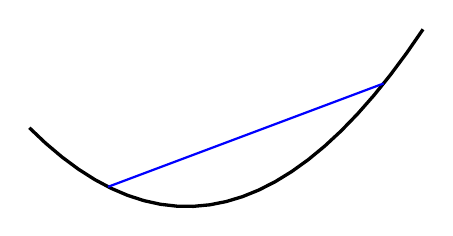
\begin{tikzpicture}
    \draw [domain=-1:4, very thick] plot (\x, {\x*\x/4 - \x/2 - 1});
    \draw [blue, thick] (0,-1) -- (3.5,0.3125);
  \end{tikzpicture}
  \caption{The graph of a convex function under its secant line (blue)}
  \label{fig:convex}
\end{figure}

Although the definition of convex functions only talks about inner division points, it is pleasant to see that this already implies continuity of such functions.
We start with the following lemma.

\begin{lem}
  Let $f : I \to \mathbb{R}$ be a convex function on an interval $I \subseteq \mathbb{R}$.
  Then
  \[
    \frac{ f(x) - f(y) }{ x - y } \leqslant \frac{ f(x) - f(z) }{ x - z } \leqslant \frac{ f(y) - f(z) }{ y - z }
  \]
  for any triplets $x, y, z \in I$ with $x < y < z$.
\end{lem}

The validity of this lemma is clear from Figure~\ref{fig:convex-secant}, when we regard all the fractions as {\em slopes} of the secant lines determined by points on the graph.
The algebraic demonstration of the above inequalities is left to the readers.

\begin{figure}
  \centering
  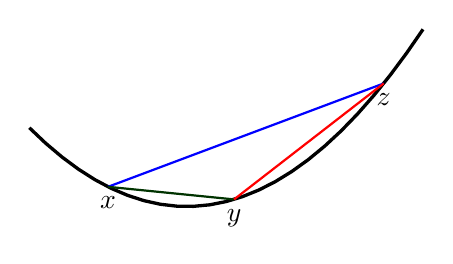
\begin{tikzpicture}
    \draw [domain=-1:4, very thick] plot (\x, {\x*\x/4 - \x/2 - 1});
    \draw [blue, thick] (0,-1) coordinate (X) -- (3.5,0.3125) coordinate (Z);
    \draw [green!20!black, thick] (X) -- (1.6, -1.16) coordinate (Y);
    \draw [red, thick] (Y) -- (Z);
    \node [below] at (X) {$x$};
    \node [below] at (Y) {$y$};
    \node [below] at (Z) {$z$};
  \end{tikzpicture}
  \caption{Comparison of slopes of secant lines on the graph of a convex function}
  \label{fig:convex-secant}
\end{figure}
\begin{thm}
  Let $I$ be a nondegenerate interval in $\mathbb{R}$, and $f : I \to \mathbb{R}$ be a convex function.
  \begin{enumerate}[$(a)$]
    \item For any $x,y$ in $I$ and $s, t \in \mathbb{R}$ with $s + t = 1$ but $s, t \notin [0,1]$, we have
      \[
	f(sx + ty) \geqslant s \, f(x) + t \, f(y), \qquad
	\text{if } sx + ty \in I.
      \]

    \item $f$ is continuous at any interior point of $I$.
  \end{enumerate}
\end{thm}

\begin{proof}
  \begin{enumerate}[$(a)$]
    \item Let $z = sx + ty$.
      By symmetry let us assume that $s < 0$ and $t > 1$.
      Then $y = \dfrac1t z - \dfrac{s}{t} x$ becomes an inner division point of $z$ and $x$ in $I$.
      From the definition of convex functions, we have
      \[
	f(y) \leqslant \frac{1}{t} f(z) - \frac{s}{t} f(x),
      \]
      which is equivalent to $f(z) = f(sx+ty) \geqslant s \, f(x) + t \, f(y)$.

    \item Let $z$ be any interior point of $I$, and fix two points $x,y \in I$ with $x < z < y$.

      Assume first that $t \in I$ and $x < t < z$.  By the definition of convex functions and (1), we have
      \begin{equation}
	\label{ineq:convex1}
	f(z) + \frac{f(x)-f(z)}{x-z} (t-z) \leqslant f(t) \leqslant
	f(z) + \frac{f(y)-f(z)}{y-z} (t-z),
      \end{equation}
      since $t$ is an inner division point of $x,z$ but an outer division point of $y,z$.  By squeeze theorem and (\ref{ineq:convex1}) we see that $f(t) \to f(z)$ as $t \to z-$.

      On the other hand, let us take $t \in I$ and $z < y < t$.
      This time the inequalities (\ref{ineq:convex1}) are reversed:
      \begin{equation}
	\label{ineq:convex2}
	f(z) + \frac{f(x)-f(z)}{x-z} (t-z) \geqslant f(t) \geqslant
	f(z) + \frac{f(y)-f(z)}{y-z} (t-z).
      \end{equation}
      Therefore $f(t) \to f(z)$ as $t \to z+$ as well,
      Since $f(z-) = f(z) = f(z+)$, we conclude that the convex function $f$ is continuous at the interior point $z$ of $I$.
  \end{enumerate}
\end{proof}

\noindent{\em Remark.}
There are a few more properties of convex functions that are related to differentiation.
They will be discussed in the later topics.

\subsection{Sup norm on continuous functions over compacts}

Let $K$ be a (nonempty) compact metric space.
Denote by $\mathcal{C}(K) = \mathcal{C}(K, \mathbb{R})$ the set of all continuous real-valued functions on $K$.

\begin{equation*}
  \| f \|_K := \sup \{ |f(x)| \colon x \in K \}.
\end{equation*}

\begin{thm}
  \label{thm:max-norm}
  \begin{enumerate}[(1)]
    \item For any $f \in \mathcal{C}(K)$, $\| f \|_K \in \mathbb{R}$.
      In fact, 
      \begin{equation}
	\label{eq:max-norm}
	\| f \|_K = \max \{ |f(x)| \colon x \in K \}.
      \end{equation}
    \item $\| \cdot \|_K$ defines a norm on $\mathcal{C}(K)$.
  \end{enumerate}
\end{thm}

\begin{proof}
  \begin{enumerate}[(1)]
    \item This follows immediately from the extreme value theorem.

    \item The first two conditions for norm are obvious.
      Let us check the triangle inequality.
      For $f, g \in \mathcal{C}(K)$, there is a point $x_0 \in K$ such that $\| f + g \|_K = |f(x_0) + g(x_0)|$.  Therefore,
      \begin{align*}
	\| f + g \|_K &= |f(x_0) + g(x_0)| \\
	&\leqslant |f(x_0)| + |g(x_0)| & \text{(This is the triangle inequality in $\mathbb{R}$)} \\
	&\leqslant \| f \|_K + \| g \|_K,
      \end{align*}
      which is needed to show.
  \end{enumerate}  
\end{proof}

This sup-norm then induces a metric, which in turn induces a topology, on $\mathcal{C}(K)$.
In general a bounded closed subset of $\mathcal{C}(K)$ is not compact.
For example, we take $K = [0,1] \subseteq \mathbb R$ and consider the sequence $\langle f_n(x) = x^n \rangle \subseteq M = \mathcal{C}(K)$.
Clearly $\| f_n \|_K = 1$ so they all belong to the unit closed ball $\overline{B_1(0)}$.
But $\langle f_n \rangle$ has no convergent subsequence under $\| \cdot \|_K$, as we shall see below.
Therefore $\overline{B_1(0)}$ in $\mathcal{C}([0,1])$ is not (sequentially) compact.

What does an open ball in $\mathcal{C}(K)$ look like?
Let $f \in \mathcal{C}(K)$ and $r > 0$.  We have
\[
  B_r(f) = \{ g \in M \colon \| g - f \|_K < r \}.
\]
The condition $\|g-f\|_K < r$ can be rephrased as
\[
  f(x) - r < g(x) < f(x) + r \qquad \forall\, x \in K.
\]
Hence $g \in B_r(f)$ means that the graph of $g$ over $K$ falls into an $r$-\textit{tubular neighborhood} of $f$, depicted as in Figure~\ref{fig:tubular}.

\begin{figure}
  \centering
  \begin{tikzpicture}
    \draw[-Stealth] (0,0) -- (5,0) node [right] {$K$};
    \draw[very thick, domain=0.5:4.5] plot (\x, {(\x-0.9)*(\x-2.5)*(\x-4)/5 + 1.5}) node [right, scale=0.7] {$f(x)$}; 
    \draw[dashed, domain=0.5:4.5] plot (\x, {(\x-0.9)*(\x-2.5)*(\x-4)/5 + 1.2}) node [right, scale=0.7] {$f(x)-r$}; 
    \draw[dashed, domain=0.5:4.5] plot (\x, {(\x-0.9)*(\x-2.5)*(\x-4)/5 + 1.8}) node [right, scale=0.7] {$f(x)+r$}; 
  \end{tikzpicture}
  \caption{A tubular neighborhood $B_r(f)$}
  \label{fig:tubular}
\end{figure}

Let us talk about convergence in $\mathcal{C}(K)$ now.
Suppose $\langle f_n \rangle$ is a Cauchy sequence in $\mathcal{C}(K)$.
Then for each $\varepsilon > 0$, there is an $N \in \mathbb{N}$ such that
\[
  \tag{2}
  |f_n(x) - f_m(x)| < \varepsilon \qquad \text{whenever $n,m \geqslant N$ and $x \in K$.}
\]
Hence the real sequence $\langle f_n(x) \rangle$ also satisfies a Cauchy condition.
By the completeness of $\mathbb{R}$, $\langle f_n(x) \rangle$ converges to some real number which we denote by $f(x)$.
We hereby write
\[
  \lim_{n \to \infty} f_n(x) = f(x), \qquad x \in K
\]
or $f_n \to f$, and call this a \textit{pointwise convergence}.
Moreover, 
\[
  \tag{3}
  \sup \{ |f_n(x) - f(x)| \colon x \in K \} \leqslant \varepsilon \qquad
  \text{whenever $n \geqslant N$},
\]
by passing $m \to \infty$.  Note that this $N$ does not depend on $x \in K$, and we call this \textit{uniform convergence} and write $f_n \rightrightarrows f$ on $K$.
We now characterize this limit function $f$ on $K$.

\begin{thm}
  \label{thm:CK-complete}
  Let $\mathcal{C}(K)$ denote the space of continuous real-valued functions defined on a compact metric space $K$.
  Let $\langle f_n \rangle \subseteq \mathcal{C}(K)$ be a Cauchy sequence under $\| \cdot \|_K$ whose pointwise limit is $f$.
  Then $f$ is also a continuous function on $K$.
\end{thm}

\begin{proof}
  Let $\varepsilon > 0$ be given.
  By (3) there is an $N \in \mathbb N$ such that
  \[
    \tag{4}
    |f_n(x) - f(x)| < \frac{\varepsilon}{3} \qquad \forall \, n \geqslant N, \, x \in K.
  \]
  Let us look at the function $f_N$.
  Since $f_N$ is continuous at any point $x \in K$, there is a $\delta > 0$ such that
  \[
    \tag{5}
    |f_N(t) - f_N(x)| < \frac{\varepsilon}{3}, \qquad \forall \, t \in K_\delta(x).
  \]
  So now whenever $t \in K_\delta(x)$, we have (by (4), (5), (4))
  \[
    |f(t) - f(x)| \leqslant |f(t) - f_N(t)| + |f_N(t) - f_N(x)| + |f_N(x) - f(x)| 
    < \frac{\varepsilon}{3} + \frac{\varepsilon}{3} + \frac{\varepsilon}{3} = \varepsilon.
  \]
  Therefore $f$ is continuous at $x \in K$.
  Since $x$ is arbitrary, we conclude that $f \in \mathcal{C}(K)$.
\end{proof}

With Theorem~\ref{thm:CK-complete}, we see that $(\mathcal{C}(K), \| \cdot \|_K)$ becomes a \textit{complete} metric space, since every Cauchy sequence in it converges to some member of it.
We will discuss more on this type of convergence towards the end of the semester.

\subsection{Normed spaces}

Let $M$ be a vector space over $F = \mathbb{R}$ or $\mathbb{C}$.
We can talk about the ``length'' of a vector in the following way.

\begin{defn}
  A \textsf{norm} on $M$ is a real-valued function $\| \cdot \|$ on $M$ that satisfies the following properties:
  \begin{enumerate}[(1)]
    \item (Positivity) $\| x \| \geqslant 0$ for any $x \in M$; moreover, $\| x \| = 0$ if and only if $x = 0$ (the additive identity in $M$).
    \item (Homogeneity) For every vector $x$ and $\alpha \in F$, we have $\| \alpha x \| = | \alpha | \, \| x \|$ (the absolute value of $\alpha$ times the norm of $x$).
    \item (Triangle inequality) For any $x, y \in M$, we have $\| x + y \| \leqslant \| x \| + \| y \|$.
  \end{enumerate}
\end{defn}

A norm $\| \cdot \|$ on $M$ can induce a metric on $M$ by setting $d(x,y) = \| x - y \|$.
The verification is immediate.
We have seen examples of normed spaces of finite dimensions.
They are: for $x = (x_1, x_2, \dots, x_m) \in \mathbb{R}^m$, define
\[
  \| x \|_p = \begin{cases}
    \left( \sum_{k=1}^m |x_k|^p \right)^{1/p}, & \text{if $1 \leqslant p < \infty$}; \\
    \max \{ |x_k| \colon k = 1, \dots, m \}, & \text{if $p = \infty$.}
  \end{cases}
\]
In fact, all of them are equivalent in the following sense.

\begin{thm}
  Let $\| \cdot \|_p$ denote the $p$-norm in $\mathbb{R}^m$, $1 \leqslant p \leqslant \infty$.
  Then for any $x \in \mathbb{R}^m$ and $1 < p < \infty$, we have
  \[
    \| x \|_\infty \leqslant \| x \|_p \leqslant \| x \|_1 \leqslant m \| x \|_\infty.
  \]
\end{thm}

The only non-trivial part of Theorem~2 is the inequality $\| x \|_p \leqslant \| x \|_1$, whose proof is left to the interested readers.
Theorem~2 implies that topology induced by $\| \cdot \|_p$ on $\mathbb{R}^m$ does not depend on $p$.
For example, the closed unit ball $\overline{B_1(0)}$ is always compact no matter which $p$-norm we choose for $M = \mathbb{R}^m$.

However, the situation is quite different for vector spaces of infinite dimensions.
Here we investigate an important instance.

\begin{defn}[$\ell^2$-space]
  Let $A$ denote the set of all infinite sequences of real numbers.
  Define
  \[
    \ell^2 = \{ \langle a_n \rangle \subseteq A \colon \sum_n |a_n|^2 < \infty \}.
  \]
  $\ell^2$ is called the space of \textsf{square-summable} sequences.\footnote{This number $2$ can be replaced by $p \in [1, \infty]$.
  We choose $p=2$ for another reason: this norm can be induced by an inner product.}
\end{defn}

In some cases $A$ might consist of infinite sequences of complex numbers, but we will not go into that.
Clearly $A$ is equipped with a structure of vector space over $\mathbb{R}$ with componentwise addition and scalar multiplication.
Here is the main result.

\begin{thm}
  The functional
  \[
    \| \langle a_n \rangle \|_2 := \left( \sum_{n=1}^\infty |a_n|^2 \right)^{1/2}
  \]
  defines a norm on $\ell^2$, and $\ell^2$ is a vector subspace of $A$.
\end{thm}

\begin{proof}
  The only non-trivial part is the triangle inequality, which we verifies as follows.  For any positive integer $m$, we have
  \[
    \left( \sum_{k=1}^m |a_k + b_k|^2 \right)^{1/2} \leqslant
    \left( \sum_{k=1}^m |a_k|^2 \right)^{1/2} +
    \left( \sum_{k=1}^m |b_k|^2 \right)^{1/2}
  \]
  (this is the triangle inequality for $2$-norm on $\mathbb{R}^m$).
  Let $m \to \infty$ and use the comparison theorem for limits, we see that
  \[
    \| \langle a_n \rangle + \langle b_n \rangle \|_2 = 
    \left( \sum_{k=1}^\infty |a_k + b_k|^2 \right)^{1/2} \leqslant
    \left( \sum_{k=1}^\infty |a_k|^2 \right)^{1/2} +
    \left( \sum_{k=1}^\infty |b_k|^2 \right)^{1/2}
    = \| \langle a_n \rangle \|_2 + \| \langle b_n \rangle \|_2,
  \]
  which is needed to show.
\end{proof}

With this theorem, $\ell^2$ is now a metric space.\footnote{Unfortunately, the topology induced by the $\ell^2$-norm is not the product topology on denumerable sets of $\mathbb{R}$'s.}
It should be noted that the closed unit ball $\overline{M_1(0)}$ is \textit{not} compact for $M = \ell^2$.
To see why, we now explain that $\overline{B_1(0)}$ is not sequentially compact.
For $i \in \mathbb{N}$, let $e_i \in \ell^2$ denote the vector with all zero entries except at the $i^\text{th}$ position, at which it is $1$.
Clearly $\langle e_i \rangle$ is a sequence in $\overline{B_1(0)}$.
But $d(e_i, e_j) = \| e_i - e_j \|_2 = \sqrt{2}$ for any $i \ne j$, hence it has no convergent subsequence.

On the other hand, $\ell^2$ has a countable subset $\ell^2(\mathbb{Q})$, consisting of all square-summable sequences with rational entries only.
It is clear that $\overline{\ell^2(\mathbb{Q})} = \ell^2$, which means that $\ell^2(\mathbb{Q})$ is a \textsf{dense} subset of $\ell^2$.
To summarize, $\ell^2$ is a \textsf{separable} space, in the sense that it has a countable dense subset.
